% latex/lz_cryo_model.tex
% Standalone TikZ rendering of the LZ cryostat radioactive model.
% Compile with: pdflatex lz_cryo_model.tex
% Then convert: pdftoppm -png -r 200 lz_cryo_model.pdf lz_cryo_model
%
% Drawn elements (radioactive / MC-active subset only):
%   * OCV outer contour: cylindrical body + 2:1 top + 2:1 bottom ellipsoidal heads
%   * ICV outer contour: cylindrical body + 2:1 top + 3:1 bottom ellipsoidal heads
%   * 5 flanges (lighter fill): OCV top reinforcing ring, OCV upper body flange pair,
%       OCV lower body flange pair, OCV bottom support flange, ICV main flange pair
%   * 6 main ports (darker fill): OCV YBe recess, OCV conduit ports, OCV tie-bar
%       ports, OCV HV port, OCV cathode-side port, OCV bottom umbilical
%
% Coordinates in cm; cathode at z=0. Drawing scale = 0.04 cm in TikZ per cm physical.

\documentclass[tikz,border=10pt]{standalone}
\usepackage{tikz}

\begin{document}
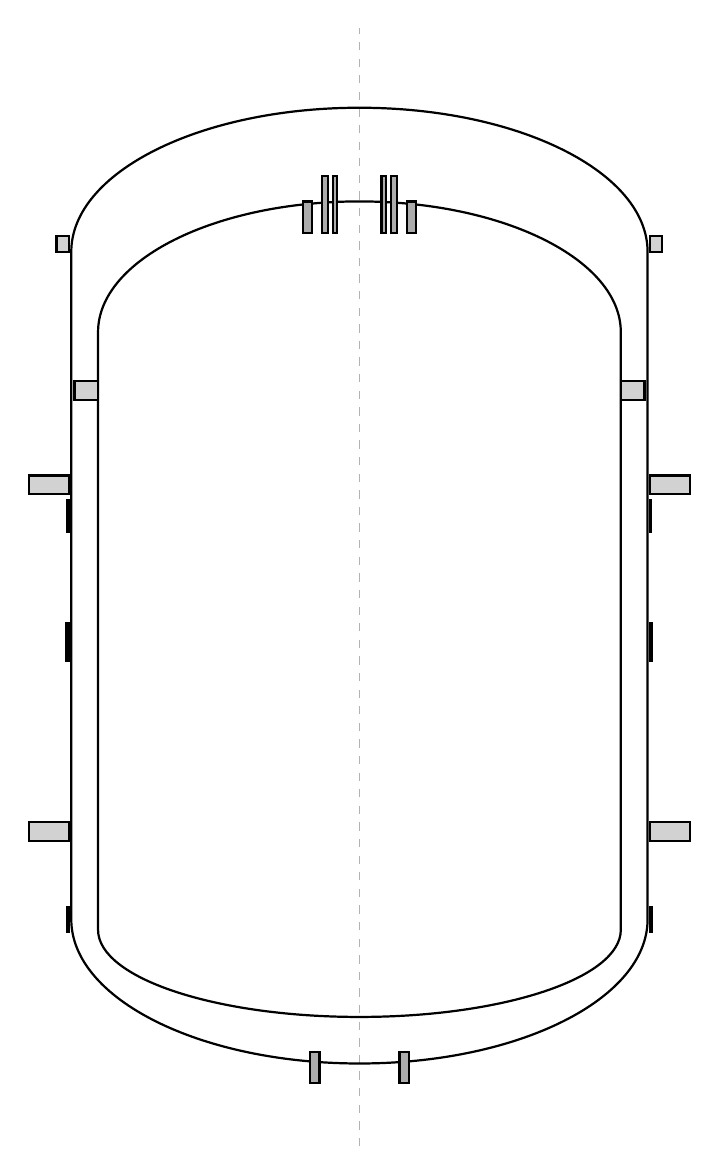
\begin{tikzpicture}[scale=0.04, line width=0.5pt]

  % ───────── Centerline (axis of symmetry) ─────────
  \draw[dashed, thin, gray!60] (0, -110) -- (0, 245);

  % ───────── OCV outer contour ─────────
  % Cylindrical body z ∈ [-38, 174], R = 91.5 cm
  % Top head: 2:1 ellipsoidal, depth = 45.75 cm, apex at z = 219.75
  % Bottom head: 2:1 ellipsoidal, depth = 45.75 cm, apex at z = -83.75
  \draw[thick]
    (91.5, -38) -- (91.5, 174)
    arc[start angle=0, end angle=180, x radius=91.5, y radius=45.75]
    -- (-91.5, -38)
    arc[start angle=180, end angle=360, x radius=91.5, y radius=45.75];

  % ───────── ICV outer contour ─────────
  % Cylindrical body z ∈ [-41.3, 148.5], R = 83 cm
  % Top head: 2:1 ellipsoidal, depth = 41.5 cm, apex at z = 190
  % Bottom head: 3:1 ellipsoidal, depth = 27.67 cm, apex at z = -68.97
  \draw[thick]
    (83.0, -41.3) -- (83.0, 148.5)
    arc[start angle=0, end angle=180, x radius=83.0, y radius=41.5]
    -- (-83.0, -41.3)
    arc[start angle=180, end angle=360, x radius=83.0, y radius=27.67];

  % ───────── Flanges (lighter fill) ─────────
  % Each flange is mirrored about the axis (left and right halves drawn)
  \foreach \s in {1,-1} {
    % OCV top reinforcing ring  (R 92.2–96.2, z 174–179)
    \draw[thick, fill=gray!35] (\s*92.2, 174) rectangle (\s*96.2, 179);
    % OCV upper body flange pair (R 92.2–105, z 97–103)
    \draw[thick, fill=gray!35] (\s*92.2, 97) rectangle (\s*105.0, 103);
    % OCV lower body flange pair (R 92.2–105, z -13–-7)
    \draw[thick, fill=gray!35] (\s*92.2, -13) rectangle (\s*105.0, -7);
    % OCV bottom support flange  (R 92.2–92.8, z -42–-34)
    \draw[thick, fill=gray!35] (\s*92.2, -42) rectangle (\s*92.8, -34);
    % ICV main flange pair       (R 83–90.5, z 127–133)
    \draw[thick, fill=gray!35] (\s*83.0, 127) rectangle (\s*90.5, 133);
  }

  % ───────── Main ports (darker fill) ─────────
  \foreach \s in {1,-1} {
    % OCV top YBe recess         (R 15–18, z 180–190)
    \draw[thick, fill=gray!65] (\s*15.0, 180) rectangle (\s*18.0, 190);
    % OCV top conduit ports x2   (R 10–12, z 180–198)
    \draw[thick, fill=gray!65] (\s*10.0, 180) rectangle (\s*12.0, 198);
    % OCV top tie-bar ports x3   (R 7–8.5, z 180–198)
    \draw[thick, fill=gray!65] (\s*7.0, 180) rectangle (\s*8.5, 198);
    % OCV HV port (side)         (R 92.2–93, z 44–56)
    \draw[thick, fill=gray!65] (\s*92.2, 44) rectangle (\s*93.0, 56);
    % OCV cathode side port      (R 92.2–92.7, z 85–95)
    \draw[thick, fill=gray!65] (\s*92.2, 85) rectangle (\s*92.7, 95);
    % OCV bottom umbilical port  (R 12.7–15.7, z -90–-80)
    \draw[thick, fill=gray!65] (\s*12.7, -90) rectangle (\s*15.7, -80);
  }

\end{tikzpicture}
\end{document}
